%%%%%%%%%%%%%%%%%%%%%%%%%%%%%%%%%%%%%%%%%%%%%%%%%%%%%%%%%%%%%%%%%%%%%%
%%  disstemplate.tex, to be compiled with latex.             %
%%  08 April 2002   Version 4                    %
%%%%%%%%%%%%%%%%%%%%%%%%%%%%%%%%%%%%%%%%%%%%%%%%%%%%%%%%%%%%%%%%%%%%%%
%%                                   %
%%  Writing a Doctoral Dissertation with LaTeX at            %
%%  the University of Texas at Austin                %
%%                                   %
%%  (Modify this ``template'' for your own dissertation.)        %
%%                                   %
%%%%%%%%%%%%%%%%%%%%%%%%%%%%%%%%%%%%%%%%%%%%%%%%%%%%%%%%%%%%%%%%%%%%%%


\documentclass[12pt]{report}    % The documentclass must be ``report''.

\usepackage{utdiss2}        % Dissertation package style file.


%%%%%%%%%%%%%%%%%%%%%%%%%%%%%%%%%%%%%%%%%%%%%%%%%%%%%%%%%%%%%%%%%%%%%%
% Optional packages used for this sample dissertation. If you don't  %
% need a capability in your dissertation, feel free to comment out   %
% the package usage command.                         %
%%%%%%%%%%%%%%%%%%%%%%%%%%%%%%%%%%%%%%%%%%%%%%%%%%%%%%%%%%%%%%%%%%%%%%

\usepackage{amsmath,amsthm,amsfonts,amscd}
                % Some packages to write mathematics.
\usepackage{eucal}      % Euler fonts
\usepackage{verbatim}       % Allows quoting source with commands.
\usepackage{makeidx}        % Package to make an index.
\usepackage{psfig}          % Allows inclusion of eps files.
\usepackage{epsfig}             % Allows inclusion of eps files.
\usepackage{citesort}           %
\usepackage{url}        % Allows good typesetting of web URLs.
\usepackage{draftcopy}     % Uncomment this line to have the
                % word, "DRAFT," as a background
                % "watermark" on all of the pages of
                % of your draft versions. When ready
                % to generate your final copy, re-comment
                % it out with a percent sign to remove
                % the word draft before you re-run
                % Makediss for the last time.



\author{Edward Amsden}    % Required

\address{305A Perkins Rd \\ Rochester, New York 14623}  % Required

\title{Push-Based Signal-Function Functional Reactive Programming}
                                                    % Required

%%%%%%%%%%%%%%%%%%%%%%%%%%%%%%%%%%%%%%%%%%%%%%%%%%%%%%%%%%%%%%%%%%%%%%
% NOTICE: The total number of supervisors and other members %%%%%%%%%%
%%%%%%%%%%%%%%% MUST be seven (7) or less! If you put in more, %%%%%%%
%%%%%%%%%%%%%%% they are put on the page after the Committee %%%%%%%%%
%%%%%%%%%%%%%%% Certification of Approved Version page. %%%%%%%%%%%%%%
%%%%%%%%%%%%%%%%%%%%%%%%%%%%%%%%%%%%%%%%%%%%%%%%%%%%%%%%%%%%%%%%%%%%%%

%%%%%%%%%%%%%%%%%%%%%%%%%%%%%%%%%%%%%%%%%%%%%%%%%%%%%%%%%%%%%%%%%%%%%%
%
% Enter names of the supervisor and co-supervisor(s), if any,
% of your dissertation committee. Put one name per line with
% the name in square brackets. The name on the last line, however,
% must be in curly braces.
%
% If you have only one supervisor, the entry below will read:
%
%   \supervisor
%       {Supervisor's Name}
%
% NOTE: Maximum three supervisors. Minimum one supervisor.
% NOTE: The Office of Graduate Studies will accept only two supervisors!
%
%
\supervisor
    {Dr. Matthew Fluet}

%%%%%%%%%%%%%%%%%%%%%%%%%%%%%%%%%%%%%%%%%%%%%%%%%%%%%%%%%%%%%%%%%%%%%%
%
% Enter names of the other (non-supervisor) members(s) of your
% dissertation committee. Put one name per line with the name
% in square brackets. The name on the last line, however, must
% be in curly braces.
%
% NOTE: Maximum six other members. Minimum zero other members.
% NOTE: The Office of Graduate Studies may restrict you to a total
%   of six committee members.
%
%
\committeemembers
%    [Erwin Schr\"odinger]
    [Arthur Nunes-Harwitt, Reader]
    {Dr. Zach Butler, Observer}
%    {Arthur Schawlow}

%%%%%%%%%%%%%%%%%%%%%%%%%%%%%%%%%%%%%%%%%%%%%%%%%%%%%%%%%%%%%%%%%%%%%%

%\previousdegrees{B.E.}
     % The abbreviated form of your previous degree(s).
     % E.g., \previousdegrees{B.S., MBA}.
     %
     % The default value is `B.S., M.S.'

%\graduationmonth{...}
     % Graduation month, either May, August, or December, in the form
     % as `\graduationmonth{May}'. Do not abbreviate.
     %
     % The default value (either May, August, or December) is guessed
     % according to the time of running LaTeX.

%\graduationyear{...}
     % Graduation year, in the form as `\graduationyear{2001}'.
     % Use a 4 digit (not a 2 digit) number.
     %
     % The default value is guessed according to the time of
     % running LaTeX.

%\typist{...}
     % The name(s) of typist(s), put `the author' if you do it yourself.
     % E.g., `\typist{Maryann Hersey and the author}'.
     %
     % The default value is `the author'.


%%%%%%%%%%%%%%%%%%%%%%%%%%%%%%%%%%%%%%%%%%%%%%%%%%%%%%%%%%%%%%%%%%%%%%
% Commands for master's theses and reports.              %
%%%%%%%%%%%%%%%%%%%%%%%%%%%%%%%%%%%%%%%%%%%%%%%%%%%%%%%%%%%%%%%%%%%%%%
%
% If the degree you're seeking is NOT Doctor of Philosophy, uncomment
% (remove the % in front of) the following two command lines (the ones
% that have the \ as their second character).
%
\degree{Master of Science} \degreeabbr{M.S.}

% Uncomment the line below that corresponds to the type of master's
% document you are writing.
%
%\masterreport
\masterthesis


%%%%%%%%%%%%%%%%%%%%%%%%%%%%%%%%%%%%%%%%%%%%%%%%%%%%%%%%%%%%%%%%%%%%%%
% Some optional commands to change the document's defaults.      %
%%%%%%%%%%%%%%%%%%%%%%%%%%%%%%%%%%%%%%%%%%%%%%%%%%%%%%%%%%%%%%%%%%%%%%
%
%\singlespacing
%\oneandonehalfspacing

%\singlespacequote
\oneandonehalfspacequote

\topmargin 0.125in  % Adjust this value if the PostScript file output
            % of your dissertation has incorrect top and
            % bottom margins. Print a copy of at least one
            % full page of your dissertation (not the first
            % page of a chapter) and measure the top and
            % bottom margins with a ruler. You must have
            % a top margin of 1.5" and a bottom margin of
            % at least 1.25". The page numbers must be at
            % least 1.00" from the bottom of the page.
            % If the margins are not correct, adjust this
            % value accordingly and re-compile and print again.
            %
            % The default value is 0.125"

        % If you want to adjust other margins, they are in the
        % utdiss2-nn.sty file near the top. If you are using
        % the shell script Makediss on a Unix/Linux system, make
        % your changes in the utdiss2-nn.sty file instead of
        % utdiss2.sty because Makediss will overwrite any changes
        % made to utdiss2.sty.

%%%%%%%%%%%%%%%%%%%%%%%%%%%%%%%%%%%%%%%%%%%%%%%%%%%%%%%%%%%%%%%%%%%%%%
% Some optional commands to be tested.                   %
%%%%%%%%%%%%%%%%%%%%%%%%%%%%%%%%%%%%%%%%%%%%%%%%%%%%%%%%%%%%%%%%%%%%%%

% If there are 10 or more sections, 10 or more subsections for a section,
% etc., you need to make an adjustment to the Table of Contents with the
% command \longtocentry.
%
%\longtocentry



%%%%%%%%%%%%%%%%%%%%%%%%%%%%%%%%%%%%%%%%%%%%%%%%%%%%%%%%%%%%%%%%%%%%%%
%   Some math support.                       %
%%%%%%%%%%%%%%%%%%%%%%%%%%%%%%%%%%%%%%%%%%%%%%%%%%%%%%%%%%%%%%%%%%%%%%
%
%   Theorem environments (these need the amsthm package)
%
%% \theoremstyle{plain} %% This is the default

\newtheorem{thm}{Theorem}[section]
\newtheorem{cor}[thm]{Corollary}
\newtheorem{lem}[thm]{Lemma}
\newtheorem{prop}[thm]{Proposition}
\newtheorem{ax}{Axiom}

\theoremstyle{definition}
\newtheorem{defn}{Definition}[section]

\theoremstyle{remark}
\newtheorem{rem}{Remark}[section]
\newtheorem*{notation}{Notation}

%\numberwithin{equation}{section}


%%%%%%%%%%%%%%%%%%%%%%%%%%%%%%%%%%%%%%%%%%%%%%%%%%%%%%%%%%%%%%%%%%%%%%
%   Macros.                              %
%%%%%%%%%%%%%%%%%%%%%%%%%%%%%%%%%%%%%%%%%%%%%%%%%%%%%%%%%%%%%%%%%%%%%%
%
%   Here some macros that are needed in this document:


\newcommand{\latexe}{{\LaTeX\kern.125em2%
                      \lower.5ex\hbox{$\varepsilon$}}}

\newcommand{\amslatex}{\AmS-\LaTeX{}}

\chardef\bslash=`\\ % \bslash makes a backslash (in tt fonts)
            %   p. 424, TeXbook

\newcommand{\cn}[1]{\texttt{\bslash #1}}

\makeatletter       % Starts section where @ is considered a letter
            % and thus may be used in commands.
\def\square{\RIfM@\bgroup\else$\bgroup\aftergroup$\fi
  \vcenter{\hrule\hbox{\vrule\@height.6em\kern.6em\vrule}%
                                              \hrule}\egroup}
\makeatother        % Ends sections where @ is considered a letter.
            % Now @ cannot be used in commands.

\makeindex    % Make the index

%%%%%%%%%%%%%%%%%%%%%%%%%%%%%%%%%%%%%%%%%%%%%%%%%%%%%%%%%%%%%%%%%%%%%%
%       The document starts here.                %
%%%%%%%%%%%%%%%%%%%%%%%%%%%%%%%%%%%%%%%%%%%%%%%%%%%%%%%%%%%%%%%%%%%%%%

\begin{document}

%\copyrightpage          % Produces the copyright page.


%
% NOTE: In a doctoral dissertation, the Committee Certification page
%       (with signatures) is BEFORE the Title page.
%   In a masters thesis or report, the Signature page
%       (with signatures) is AFTER the Title page.
%
%   If you are writing a masters thesis or report, you MUST REVERSE
%   the order of the \commcertpage and \titlepage commands below.
%
\commcertpage           % Produces the Committee Certification
            %   of Approved Version page (doctoral)
            %   or Signature page (masters).
            %       20 Mar 2002 cwm

\titlepage              % Produces the title page.



%%%%%%%%%%%%%%%%%%%%%%%%%%%%%%%%%%%%%%%%%%%%%%%%%%%%%%%%%%%%%%%%%%%%%%
% Dedication and/or epigraph are optional, but must occur here.      %
%%%%%%%%%%%%%%%%%%%%%%%%%%%%%%%%%%%%%%%%%%%%%%%%%%%%%%%%%%%%%%%%%%%%%%
%
%\begin{dedication}
%\index{Dedication@\emph{Dedication}}%
%Dedicated to my wife Shirley.
%\end{dedication}


\begin{acknowledgments}     % Optional
\index{Acknowledgments@\emph{Acknowledgments}}%
I wish to thank the multitudes of people who helped me. Time would
fail me to tell of \ldots
\end{acknowledgments}


% The abstract is required. Note the use of ``utabstract'' instead of
% ``abstract''! This was necessary to fix a page numbering problem.
% The abstract heading is generated automatically.
% Do NOT use \begin{abstract} ... \end{abstract}.
%
\utabstract
\index{Abstract}%
\indent
%\begin{abstract}
Functional Reactive Programming is a promising \new{approach} 
\rn{systems -- seems weird to identify it with the implementations... model, approach?} 
for writing interactive and time-dependent programs. Signal-function FRP 
is variant of FRP 
% a subclass of these systems 
which provides advantages in modularity and correctness, but
has proven difficult to implement efficiently.

\textred{The abstraction of signal vectors provides the necessary type apparatus to
distinguish components of the input and output of signal functions which benefit
from a push-based implementation from those which benefit from a pull-based
implementation, and to combine both implementation strategies in a single system.}

\rn{Without understanding it a priori, the above para is hard to
  parse.  How about the following?}

\new{One important implementation trade-off is whether evaluation 
% of a composition 
of signal functions is {\em push-based} or {\em pull-based}.
The {\em signal-vector} technique addresses this by providing a type-level
  description of the inputs and outputs of signal functions, 
  distinguishing} components that benefit from a push-based
implementation from those that benefit from a pull-based
implementation.  This makes it possible to combine both implementation
strategies in a single system.

We describe a \new{novel} \rn{is it novel? how? need clear contributions}
 signal-function FRP system which provides push-based evaluation
for events, pull-based evaluation for signals, and a simple monadic evaluation
interface that permits the system to easily integrate with one or more
IO systems.
\end{abstract}




\tableofcontents   % Table of Contents will be automatically
                   % generated and placed here.

\listoftables      % List of Tables and List of Figures will be placed
\listoffigures     % here, if applicable.



%%%%%%%%%%%%%%%%%%%%%%%%%%%%%%%%%%%%%%%%%%%%%%%%%%%%%%%%%%%%%%%%%%%%%%
% Actual text starts here.                       %
%%%%%%%%%%%%%%%%%%%%%%%%%%%%%%%%%%%%%%%%%%%%%%%%%%%%%%%%%%%%%%%%%%%%%%
%
% Including external files for each chapter makes this document simpler,
% makes each chapter simpler, and allows for generating test documents
% with as few as zero chapters (by commenting out the include statements).
% This allows quicker processing by the Makediss command file in case you
% are not working on a specific, long and slow to compile chapter. You
% can even change the chapter order by merely interchanging the order
% of the include statements (something I found helpful in my own
% dissertation).
%

%\begin{abstract}
Functional Reactive Programming is a promising \new{approach} 
\rn{systems -- seems weird to identify it with the implementations... model, approach?} 
for writing interactive and time-dependent programs. Signal-function FRP 
is variant of FRP 
% a subclass of these systems 
which provides advantages in modularity and correctness, but
has proven difficult to implement efficiently.

\textred{The abstraction of signal vectors provides the necessary type apparatus to
distinguish components of the input and output of signal functions which benefit
from a push-based implementation from those which benefit from a pull-based
implementation, and to combine both implementation strategies in a single system.}

\rn{Without understanding it a priori, the above para is hard to
  parse.  How about the following?}

\new{One important implementation trade-off is whether evaluation 
% of a composition 
of signal functions is {\em push-based} or {\em pull-based}.
The {\em signal-vector} technique addresses this by providing a type-level
  description of the inputs and outputs of signal functions, 
  distinguishing} components that benefit from a push-based
implementation from those that benefit from a pull-based
implementation.  This makes it possible to combine both implementation
strategies in a single system.

We describe a \new{novel} \rn{is it novel? how? need clear contributions}
 signal-function FRP system which provides push-based evaluation
for events, pull-based evaluation for signals, and a simple monadic evaluation
interface that permits the system to easily integrate with one or more
IO systems.
\end{abstract}

%\chapter{Introduction}
\label{chapter:Introduction}

Most of the useful programs which programmers are asked to write must react to inputs which are not available at the time the program starts,
and produce effects at many different times throughout the execution of the program. Examples of these programs include GUI applications,
web browsers, web applications, video games, multimedia authoring and playback tools, operating system shells and kernels, servers,
robotic control programs, and many others. This attribute of a program is called reactivity.

Functional reactive programming (FRP) is a promising class of abstractions for
writing interactive programs in functional languages. The FRP abstractions are
{\em behaviors} (also termed {\em signals}), which are functions of continuous
time, and {\em events}, which are sequences of time-value pairs. These
abstractions translate desirable properties of the underlying functional
languages, such as higher-order functions and referential transparency, to
reactive constructs, generally without modifications to the underlying language.
This permits the compositional construction of reactive programs in purely
functional languages.

Functional reactive programming was introduced, though not quite by name, with
Fran~\cite{Elliott1997}, a compositional system for writingm reactive
animations. From the start, two key challenges emerged: the enforcement of
{\em causality}\footnote{Causality is the property that a value in an FRP
program depends only on present and past values. Obviously, a program which
violates this property is impossible to evaluate, but in some FRP systems such
programs are unfortunately quite easy to write down.} in FRP programs, and the
efficient evaluation of FRP programs.

The first challenge was addressed by representing FRP programs, not as
compositions of behaviors and events, but as compositions of transformers of
behaviors and events called {\em signal functions}. By not permitting direct
access to behaviors or events, but representing them implicitly, signal
functions prohibit accessing past or future time values, only allowing access to
values in the closure of the signal function and current input values. Signal
function FRP programs are written by composing signal functions, and are
evaluated using a function which provides input to the signal function and acts
on the output values. This evaluation function is generally elided in existing
literature on signal functions, but we provide a documented and improved
interface for evaluating signal functions. A further advantage of
signal-function FRP programs is that they are more readily composed,
since additional signal functions may be composed on the input or output side of
a signal function, rather than simply the output side as in classic
(non-signal-function) FRP systems.

The second challenge was addressed for classic FRP by the creation of a hybrid
push-pull FRP system~\cite{Elliott2009}. This system relied on the distinction
between reactivity and time dependence to decompose behaviors into phases of
constant or simply time-dependent values, with new phases initiated by event
occurrences. However, this implementation did not address concerns of causality
or composability. Further, the existence of events as first-class values in
classic FRP forced the use of an impure and resource-leaking technique to
compare events when merging, in order to determine which event had the first
occurrence after the current time. Further, since the classic FRP interface
permits access to only the output of a behavior or event, and is always bound to
its implicit inputs, the best the push-based implementation can do is to block
when no computation needs to be performed. The computation cannot be suspended
entirely as a value representation.

To address both challenges in a FRP implementation, we combine the approaches
and demonstrate a push-pull signal-function FRP system. The current
implementation approach for signal-function FRP is inherently
pull-based~\cite{Nilsson2002}, but recent work on N-ary
FRP~\cite{Sculthorpe2011}, a variant of signal-function FRP which enumerates
inputs and distinguishes between events and behaviors, provides a representation
which suggests a method of push-based evaluation. In previous implementations of
signal-function FRP, events were simply option-valued behaviors. This approach has
the advantage of being simple to implement. However, it does not have an obvious
semantics for event merging. Further, it necessitates pull-based evaluation,
since there is no way to separate the events which may be pushed from the truly
continuous values which must be repeatedly sampled.

This thesis describes the design and implementation of TimeFlies, a push-pull signal-function FRP system. This system is presented as a library
of combinators for constructing and evaluating FRP programs.

%\chapter{Background}
\label{chapter:Background}

The key abstraction of functional programming is the function, which takes an input and produces an output. Functions may produces functions
as output and/or take functions as input. We say that functions are {\em first-class values} in a language.

Most reactive programs are written in an imperative style, using low-level and non-composable abstractions including callbacks
or object-based event handlers, called by event loops. This ties the model of interactivity to low-level implementation details such as timing and event handling models. 

FRP implies that a model should keep the characteristics of functional programming (i.e. that the basic constructs of the language
should remain first-class) while incorporating reactivity into the language model. In particular, functions should be lifted to operate on reactive values,
and functions themselves ought to be reactive.

The goal of FRP is to provide compositional and high-level abstractions for creating reactive programs. The key
abstractions of FRP are behaviors or signals\footnote{Behaviors are generally referred to as {\em signals} in signal function literature. This is unfortunate, since a signal
function may operate on events, signals, or some combination of the two.}, which are time-dependent values defined at every point in continuous time, and events, which are 
values defined at countably many points in time. An FRP system will provide functions to manipulate events and signals and to react
to events by replacing a portion of the running program in response to an event. Behaviors and events, or some abstraction
based on them, will be first class, in keeping with the spirit of functional programming. Programs implemented in functional reactive
models should of course be efficiently executable. This has proven to be the main challenge in implementing Functional Reactive Programming.

The two general approaches to FRP are ``classic'' FRP, where behaviors and signals are first-class and reactive objects, and ``signal-function'' FRP,
where transformers of signals and events are first-class and reactive objects.

\section{Classic FRP}
\label{section:Background-classic_frp}

The first FRP system, Fran~\cite{Elliott1997}, was introduced as a system for compositionally describing interactive animations.
Though the term ``Functional Reactive Programming'' was not used in this work, it was the first to introduce the concept of first-class
behaviors and events as an abstract model for reactive programs. The key motivation was to separate the implementation of reactivity
from the modelling of reactivity, so that a programmer could be freed from details such as sampling time-varying values, time-slicing
to simulate updating values in parallel, and sampling of inputs.

The first implementation of FRP outside the Haskell language was Frapp\'{e}, an FRP implementation for the Java Beans framework. Frapp\'{e} built on
the notion of events and {\em bound properties} in the Beans framework, providing abstract interfaces for FRP events and behaviors, and combinators
as concrete classes implementing these interfaces. The evaluation of Frapp\'{e} used Bean components as sources and sinks, and the implementation of
Bean events and bound properties to propagate changes to the network~\cite{Courtney2001-2}.


The FrTime\footnote{FrTime is available in the current version of Dr Racket (5.2.1).}~\cite{Cooper2006} language extends the Scheme evaluator with a mutable
dependency graph, which is constructed by program evaluation. This graph is then updated by signal changes. FrTime does not provide a distinct concept of
events, and chooses branches of the dependency graph by conditional evaluation of signals, rather than by the substitution of signals used by FRP systems.

The Reactive~\cite{Elliott2009} system is a push-based FRP system with first-class behaviors and events. The primary insight of Reactive is
the separation of reactivity (or changes in response to events whose occurrence time could not be know beforehand) from time-dependence. This
gives rise to {\em reactive normal form}, which represents a behavior as a constant or simple time-varying value, with an event stream carrying values
which are also behaviors in reactive normal form. Push-based evaluation is achieved by forking a Haskell thread to evaluate the head behavior,
while waiting on the evaluation of the event stream. Upon an event occurrence, the current behavior thread is killed and a new thread
spawned to evaluate the new behavior. Unfortunately, the implmentation of Reactive uses a tenuous technique which depends on also forking threads to evaluate
two haskell values concurrently in order to implement event merging. This relies on the library author to ensure consistency when this technique is
used, and leads to thread leakage when one of the merged events is itself the merging of other events.

The reactive-banana~\cite{Apfelmus} library is a push-based FRP system designed for use with Haskell GUI frameworks. In particular, it features a monad for
the creation of behaviors and events which may then be composed and evaluated. This monad includes constructs for binding GUI library constructs to primitive events.
It must be ``compiled'' to a Haskell IO action for evaluation to take place. The implementation of reactive-banana is similar to FrTime, using a dependency graph to update the network on event occurences. Reactive-banana eschews generalized switching in favor of branching functions on behavior values, similarly to FrTime, but
maintains the distinction between behaviors and events. Rather than a generalized switching combinator which allows the replacement of arbitrary behaviors,
reactive-banana provides a step combinator which creates a stepwise behavior from the values of an event stream.

A recent thesis~\cite{Czaplicki2012} described Elm, a stand-alone language for reactivity. Elm provides combinators for manipulating discrete events, and
compiles to Javascript, making it useful for client-side web programming. However, Elm does not provide a notion of switching or of continuous time behaviors,
though an approximation is given using discrete-time events which are actuated at repeated intervals specified during the event definition. The thesis asserts
that Arrowized FRP (signal-function FRP, Section~\ref{section:Background-signal_function_frp}) can be embedded in Elm, but provides no support for this assertion.

\section{Signal Function FRP}
\label{section:Background-signal_function_frp}

An alternative approach to FRP was first proposed in work on Fruit~\cite{Courtney2001-1}, a library for declarative specification of GUIs. This library
utilized the abstraction of Arrows~\cite{Hughes2000} to structure {\em signal functions}. Arrows are abstract type constructors with input and output type
parameters, together with sequential ({\tt >>>}) and parallel ({\tt first} and {\tt second}) composition, branching ({\tt ***}), and lifting ({\tt arr}) functions
to the Arrow type. Signal functions are the first-class abstraction in this approach, they represent time-dependent and reactive transformers of events and signals, 
which are themselves not first class, since such values cannot be directly manipulated by the programmer.
This approach has two motivations: it increases modularity since both the input and output of signal functions may be transformed,
as opposed to signals or events which may only be transformed in their output, and it avoids a large class of time and space leaks which have emerged when
implementing FRP with first-class signals and events.

Similarly to FrTime, the netwire~\cite{Soylemez} library eschews dynamic switching, in this case in favor of {\em signal inhibition}. Netwire is written as an arrow
transformer, which, together with the Kliesli arrow instance for the IO monad\footnote{Any monad forms a Kliesli arrow.}, permits it to lift IO actions as sources and
sinks at arbitrary points in a signal function network. Signal inhibition is accomplished by making the output of signal functions a monoid, and then combining the
outputs of signal functions. An inhibited signal function will produce the monoid's zero as an output. Primitives have defined inhibition behavior, and composed signal
functions inhibit if their outputs combine to the monoid's zero.

Yampa~\cite{Nilsson2005} is an optimization of the Arrowized FRP system first utilized with Fruit (see above). The implementation of Yampa makes use of Generalized Algebraic Datatypes to permit a much larger class of type-safe datatypes for the signal function representation. This representation, together with ``smart''
constructors and combinators, enables the construction of a self-optimizing arrowized FRP system. Unfortunately, the primary inefficiency, that of unnecessary evaluation
steps due to pull-based evaluation, remains. Further, the optimization is ad-hoc and each new optimization requires the addition of new constructors, as well
as the updating of every primitive combinator to handle every combination of constructors. However, Yampa showed noticeable performance gains over previous Arrowized FRP implementations.

A recent PhD thesis~\cite{Sculthorpe2011} introduced N-Ary FRP, a technique for typing Arrowized FRP systems using dependent types. The bulk of the work consisted
in using the dependent type system to prove the correctness of the FRP system discussed. This work introduced the typing construct of signal vectors,
which permit the distinction of signal and event types at the level of the FRP system, instead of making events merely a special type of signal.

\section{Outstanding Challenges}
\label{section:Background-outstanding_challenges}

At present, there are two key issues apparent with FRP. First, while signal-function FRP is inherently safer and more modular than classic FRP, it has yet to be
efficiently implemented. Second, the interface between FRP programs and the many different sources of inputs and sinks for outputs available to a modern application
writer remains ad-hoc and is in most cases limited by the implementation. One key exception to this is the reactive-banana system, which provides a monad for
constructing primitive events and behaviors from which an FRP program may then be constructed. However, this approach is still inflexible as it requires library support
for the system which the FRP program will interact with. Further, classic FRP programs are vulnerable to time leaks and violations of causality due to the ability
to directly manipulate reactive values.

%\section{Semantics}
\label{section:semantics}
%\section{Implementation}
\label{section:Implementation}

We now turn our attention to the implementation of the signal function
system. We will discuss representations of inputs, outputs, and signal functions,
as well as the implementations of specific signal function combinators.

\subsection{Signal Functions}
\label{subsection:Implementation-Signal_Functions}

The design of signal functions specifies a family of types for the inputs and
outputs of signal functions. Signal functions are not functions in the purest
sense, however. They are not mappings from a single instance of their input
type to a single instance of their output type. They must be implemented with
respect to the temporal semantics of their inputs and outputs.
\rn{What does that mean?  ``implement with respect to the temporal
  semantics'' seems like an underspecified relation.  I'm also not
  sure about the use of ``purest'' -- isn't this a semantics
  vs. runtime/implementation issue?}

We therefore start by creating a set of concrete datatypes for the inputs and
outputs of signal functions. These datatypes will be parameterized by the input
and output types of the signal function, and will not be exposed to the user of
the library. Rather, they will specify how data is represented during the
temporal evaluation of signal functions. 
\rn{Maybe ``temporal evaluation'' could be more concrete... this means
  repeated running sampling computation, right?  Maybe there should be a term
  for each sampling interval, epoch, whatever?}
We then implement signal functions
as records of functions from these concrete types \textred{to these concrete types} paired
with new signal functions. The evaluation system for signal functions then
maintains this record for the signal function it is evaluating, calls the
correct function for the current input, actuates the outputs (using supplied
functions from the outputs to monadic actions) and replaces the record with the
newly supplied signal function record.

In Section~\ref{section:System_Design_and_Interface} we presented signal vectors
as a set of types. In order to be completely principled, we should isolate these
types into their own {\em kind} (a sort of type of types); however, the Haskell
extension for this was far from stable at the time this system was created.
\rn{This should probably be a footnote... doesn't need to be highlighted.}

Using the Glasgow Haskell Compiler's extension for Generalized Algebraic
Datatypes~\cite{Cheney2003,Xi2003,PeytonJones2006}, we specify three concrete
datatypes which are parameterized over signal vectors, and represent
information about \textred{one} temporal point \rn{and not others?
  rephrase?} in a signal function's evaluation.

The first type carries the instantaneous values of all signals in a signal vector.
There is precisely one constructor for each type constructor of a signal vector ({\tt SVEmpty},
{\tt SVSignal}, {\tt SVEvent}, and {\tt SVAppend}). The constructor for {\tt SVSignal}
carries a value typed with the type parameter of the {\tt SVSignal} constructor,
the rest do not. Thus, in this representation, for any signal vector, there is
a node in the representation for each node in the signal vector, and precisely
the signal nodes have values.

The next representation contains a constructor for {\tt SVEvent} nodes, carrying
a value typed by the type parameter of {\tt SVEvent}, and two constructors, each
of which carries a representation for one child of a {\tt SVAppend} node (the
left or right), and is parametric in the other. \rn{?? Example?} Thus, an instance of this
representation is a path from the root of a signal vector to an event node,
carrying exactly one value for the event.

The last representation is used for efficient implementation, and has three
constructors. One constructor represents a {\tt SVSignal} node and has a value
typed by its type parameter. The second carries representations of both
children of a {\tt SVAppend} node. The third is parametric in its signal vector,
and thus represents the absence of information for an arbitrary signal vector.
This representation contains values for all, some, or none of the {\tt SVSignal}
nodes of a signal vector.

Signal functions are implemented by combining two strategies for temporal
updates. The first such strategy is sampling. A signal function has a 
continuation which may be invoked at regular intervals, using the partial
representation of signals described above as input and producing such a
representation as output. This amounts to repeated sampling of the output
signals of a signal function.

The other approach is notification. Signal functions have a second continuation
which is only invoked when there is an event occurence on their input. The input
to this continuation is, of course, the representation of event occurrences. If
events were signals, they would be sampled as above, and the sampling interval
would not match the event occurrence interval. It would thus be necessary to
represent these non-occurrences. By implementing event handling separately from
signal updates, we eliminate the need for a representation of event
non-occurences and the need for invoking event-handling code at every time step.

We represent signal functions as a GADT with three type parameters and two 
constructors. The first type parameter represents the initialization state,
and is specialized to {\tt Initialized} or {\tt NonInitialized} depending on the
constructor. It would of course be possible to represent these as two distinct
datatypes, but this representation communicates the intuition that these are
two states of the same object, rather than separate objects. The other two type
parameters are the input and output signal vectors, respectively. The signal
functions that a user will compose are non-initialized signal functions.
They must be provided with an initial set of input signal values, which are considered
the sample for time zero, and represented by the full representation of signals
described above. When provided with this input, they produce their time-zero
output and an initialized signal function.

Initialized signal functions carry the two continuations described above.
The first continuation takes a time differential and a set of signal updates
(the partial representation of signals) and returns a set of signal updates, a
collection of event occurrences, and a new initialized signal function of the
same type. This is the continuation called when sampling.

The second continuation takes an event occurrence, and returns a collection of
event occurrences and a new signal function of the same type. This continuation
is only called when there is an event occurrence to be input to the signal
function.

This is the \textred{type and} framework for our signal function implementation.
Combinators are implemented as functions which return these types with specific
implementations of the continuations. Space precludes a full discussion of the
implemenation of each combinator, but some of the examples will be discussed.

The simplest example of the implementation of is the {\tt identity} combinator.
This signal function
simply passes all of its inputs along as outputs. The initialization function
simply passes along the received sample and outputs the initialized version of
the signal function. The initialized version of the input is similar, but is
self-referential. It outputs itself as its replacement. This is standard for
simple and routing combinators which are not reactive, and simply re-arrange,
discard, or combine signals and events.

In order for our primitive signal functions to be useful, we need a means of
composing them. Serial composition creates one signal function from two, by
using the output of one as the input of the other. The serial composition
combinator is styled {\tt (>>>)}. The implementation of this operator is one
place where the advantage of responding to events independently from signal
samples becomes clear. 

This is the only primitive combinator which takes two signal functions, and
thus, it is the only way to combine signal functions. Parallel, branching, and
joining composition can be achieved by modifying signal functions with the
{\tt first} and {\tt second} combinators and composing them with the
routing and joining combinators.

Combinators which take one or more signal functions as input must recursively
apply themselves, as is shown in the implementation of serial composition.
They must also
handle initialization, retaining the initialized signal functions and passing
them to the initialized version of the combinator.

The switch combinator is the means of introducing reactivity into a signal
function. This combinator allows a signal function to replace itself by
producing an event occurrence. The combinator wraps a signal function, and 
observes an event on the right side of the output signal vector. At the first
occurrence of the event, the signal function carried by the occurrence replaces
the signal function. 

The switch combinator stores the input sample provided during initialization,
and updates it with the input signal updates. When the wrapped signal function
produces an occurrence carrying a new signal function, that signal function is
initialized with the stored input sample. It is then "wrapped" by another
function which closes over its output sample, and outputs the sample as a signal
update as the next time step. After this, it acts as the new signal function.
This wrapping has some performance implications, which are discussed in Section~\ref{section:Discussion}.

This combinator checks the outputs of the wrapped
signal function for an event occurrence from which an uninitialized signal
function is extracted. The switch combinator stores the full sample
for its input vector (which is identical to the input vector of the supplied
signal function) to initialize the new signal function. This also demands that
it add a wrapper to the new signal function which waits for the next sampling
interval and actuates the sample output at initialization as an output set
of changes to the signal. This has some performance implications, which are
discussed in Section~\ref{section:Discussion}.

Most of the routing combinators are simple to implement. The only task is to add
remove, or replace routing constructors on signal updates and event occurrences.
Since these signal functions are stateless and primitive, they can simply
return themselves as their replacements.

The looping feedback combinator is particularly tricky. As it is currently
implemented, the initial sample for the right side of the input signal vector to
the supplied function is the right side of the output sample. This is acceptable,
given Haskell's non-strict evaluation strategy, but it is necessary that the
right side of the signal function's output not be immediately dependent on its
input. The feedback combinator makes use of Haskell's lazy evaluation to
feed events back into the combinator, and stores signal updates until the next
sample. Signal samples are thus automatically decoupled after initialization.
The implementation makes use of the recursive nature of the {\tt let} construct
in Haskell, and the non-strict evaluation of Haskell, to implement feedback.

Time dependence is introduced by the {\tt time}, {\tt delay}, and {\tt integrate}
combinators. The time combinator simply sums the time updates and provides the
sum as a signal output. The {\tt delay} combinator keeps a table of events
which have come in, along with their schedule occurrence time, and produces
them as output when time advances far enough. The integrate combinator performs
rectangle-rule integration on signal samples with respect to
time. \rn{repetitive with previous section...}

The implementation strategy leaves room for optimizations. In particular, an
additional constructor for time-independent signal functions would allow
portions of a signal function to forgo evaluation during time steps unless they
had signal updates. Optimizations in the style of Yampa, observed by keeping
an updated AST for the signal function and pattern-matching on it when switching,
might further improve performance. In particular, collapsing nested or
serially-composed versions of the {\tt switchWait} step when switching would
remove at least some of the observed dependence of performance on sampling rate.
Nevertheless, this implementation performs quite well as it currently exists, as
we demonstrate in Section~\ref{section:Discussion}.

\subsection{Evaluation Interface}
\label{subsection:Implementation-Evaluation_Interface}
The evaluation interface provides the means of evaluating a signal function
with inputs and producing effects in response to the signal function's outputs.
We would like to produce a set of constructs that interacts well with Haskell's
system for external IO.

The evaluation interface translates between signal functions and the standard
Haskell construct for sequencing effects and external inputs, namely,
{\em monads}~\cite{PeytonJones1993}. The inspiration for monads is drawn from
the rather esoteric domain of category theory, but the concept as applied to
programming languages is actually rather simple.

By formulating
the evaluation interface as a monad transformer, we need only define the
operations relevant to the evaluation of signal functions, and we can depend
on the constructs of the IO monad to interact with whatever inputs and outputs
are necessary. In some cases, we may not wish to use the IO monad at all (e.g
for testing or simulation). In this case, we can parameterize over another
monad, such as the Identity monad (which has no special operations and whose
context is just the value), or the State monad (which maintains an implicit 
state accessible by {\tt get} and {\tt put} operations).

The {\tt SFEvalState} type constructor parameterizes over input types for signal
functions, and underlying monads for a monad transformer, but is not itself
a monad transformer. It describes the state of signal function evaluation.
It consists of a record with four members: the current signal function,
the set of handlers for outputs, the current input signal delta, and the last
sample time.

The {\tt SFEvalT} monad transformer does not make the {\tt get} and {\tt put}
actions available, but uses them in its implementation of the {\tt push},
{\tt update}, and {\tt sample} actions.

The {\tt push} action pushes an event onto the input of the signal function,
resulting in immediate evaluation of the relevant components signal function
and possible actuation of handlers specified for output events. It is
implemented by fetching the {\tt SFEvalState}, applying the event continuation
of the signal function contained by the {\tt SFEvalState} to the pushed event,
thus obtaining a new signal function and a list of events, applying the handlers
contained in the {\tt SFEvalState} to the output events, replacing the signal
function in the {\tt SFEvalState}, and replacing the {\tt SFEvalState}.

The {\tt update} action modifies the current input signal update, which will be
sampled at the next {\tt step} action. It has no immediately observable effect.
It simply updates the value of one signal in the input signal vector.

The {\tt step} action takes a time delta, and calls the signal continuation of
the stored signal function with the time delta and the stored signal update. It
actuates the outputs using the stored handlers, replaces the stored delta with
an empty delta, and stores the resulting new signal function in the state.

%\chapter{Evaluation and Comparisons}
\label{chapter:Evaluation_and_Comparisons}

We have described the implementation of a push-pull signal-function FRP system.
Push-based event evaluation should have advantages in event latency and overall
performance over pull-based event evaluation. We would also like to compare
the evaluation interface in the current widely-used system with the one proposed
here, again in order to verify that the theoretical benefits do appear in
practice.

One way to evaluate this is to write an application in two systems, and benchmark
these systems for comparison. In order to compare TimeFlies with Yampa, the most
recently released pull-based signal-function FRP system, we decided to implement
a suitable application in both.

\section{Methodology and Results}
\label{section:Evaluation_and_Comparisons-Methodology_and_Results}

The example application from Chapter~\ref{chapter:Example_Application}, an
OpenFlow controller, was also implemented in Yampa. A slightly-modified
TimeFlies implementation, which used a polling loop rather than the GHC event
system to obtain events, but still ``pushed'' events to TimeFlies once they were
acquired, was also implemented.

These three controllers were benchmarked using the {\tt cbench}
program~\cite{cbench}. The amount to time to pause between time and signal
updates (the inverse of the sampling rate for signals) was passed as a parameter
to each program. The {\tt cbench} benchmark operates by sending a simulated
packet-in event, waiting for a rule response, and then repeating. The output of
the benchmark is the number of times this occurs in a second. This is thus a
test of event latency in a reactive system.

Figure \ref{fig:timeflies-yampa-comparison} shows the performance comparison.
Toward the left of the graph is lower pause times (more frequent sampling). The
y-axis is a higher rate of responses (higher numbers are preferred). 

\begin{figure}
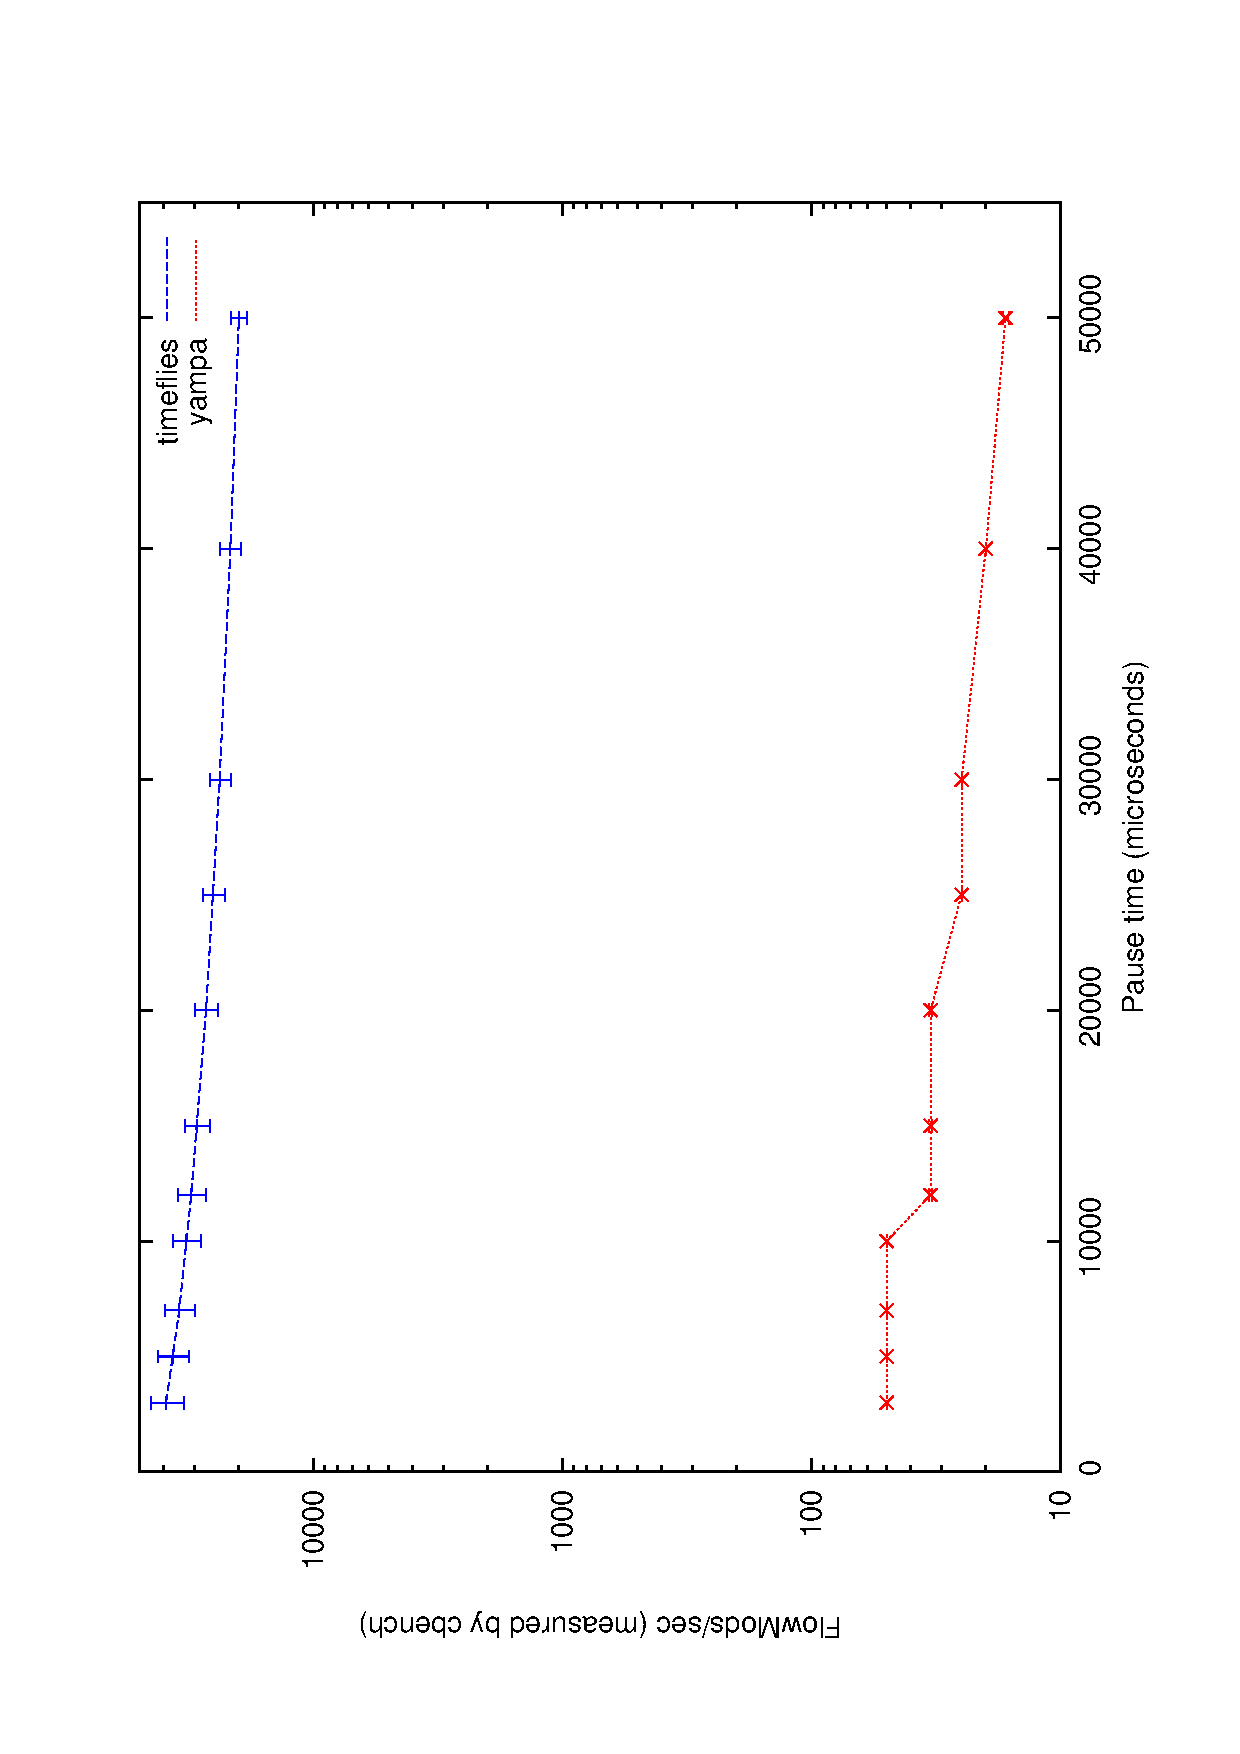
\includegraphics{graph}
\hrule
\caption{Comparison of timeflies vs. Yampa implementing an OpenFlow learning switch controller.}
\label{fig:timeflies-yampa-comparison}
\end{figure}

There is some correlation between the sampling rate and the response rate
for TimeFlies, which is due to the continued wrapping of a replacement signal
function by {\tt switch} until the next time step (see Section~\ref{subsection:Implementation-Signal_Functions-Implementation_of_Signal_Function_Combinators}).
Nevertheless, TimeFlies outperforms Yampa in event response by several orders of magnitude,
even at a very high sampling rate. This is due to two factors. First, TimeFlies can react
to individual events without evaluating the whole signal function. Second, in
the implementation described in Chapter~\ref{chapter:Example_Application}, the
interface of TimeFlies permits us to connect its evaluation directly to GHC's
event manager, while the design of Yampa requires us to use threads and
synchronized communication\footnote{Yampa does include a step-wise evaluation
function, but it still couples event evaluation firmly to time steps, and is not well
documented.}. Even the TimeFlies implementation using polling IO outperforms the
Yampa version, due to the ability to evaluate multiple events per time step.


%\include{conclustion.tex}
%\section{Ongoing and Further Work}
\label{section:ongoing_and_further_work}


%%%%%%%%%%%%%%%%%%%%%%%%%%%%%%%%%%%%%%%%%%%%%%%%%%%%%%%%%%%%%%%%%%%%%%
% Appendix/Appendices                                                %
%%%%%%%%%%%%%%%%%%%%%%%%%%%%%%%%%%%%%%%%%%%%%%%%%%%%%%%%%%%%%%%%%%%%%%
%
% If you have only one appendix, use the command \appendix instead
% of \appendices.
%
%\appendices
%\index{Appendices@\emph{Appendices}}%

%\include{chapter-appendix1}

%\include{chapter-appendix2}

%\include{chapter-appendix3}


%%%%%%%%%%%%%%%%%%%%%%%%%%%%%%%%%%%%%%%%%%%%%%%%%%%%%%%%%%%%%%%%%%%%%%
% Generate the bibliography.                         %
%%%%%%%%%%%%%%%%%%%%%%%%%%%%%%%%%%%%%%%%%%%%%%%%%%%%%%%%%%%%%%%%%%%%%%
%                                    %
% NOTE: For master's theses and reports, NOTHING is permitted to     %
%   come between the bibliography and the vita. The command      %
%   to generate the index (if used) MUST be moved to before      %
%   this section.                            %
%                                    %
%
\nocite{*}      % This command causes all items in the           %
                % bibliographic database to be added to          %
                % the bibliography, even if they are not         %
                % explicitly cited in the text.              %
        %                            %
  % Here the bibliography           %
        % is inserted.                %

\index{Bibliography@\emph{Bibliography}}%
\bibliographystyle{plain}
\bibliography{thesis}
%%%%%%%%%%%%%%%%%%%%%%%%%%%%%%%%%%%%%%%%%%%%%%%%%%%%%%%%%%%%%%%%%%%%%%


%%%%%%%%%%%%%%%%%%%%%%%%%%%%%%%%%%%%%%%%%%%%%%%%%%%%%%%%%%%%%%%%%%%%%%
% Generate the index.                            %
%%%%%%%%%%%%%%%%%%%%%%%%%%%%%%%%%%%%%%%%%%%%%%%%%%%%%%%%%%%%%%%%%%%%%%
%                                    %
% NOTE: For master's theses and reports, NOTHING is permitted to     %
%   come between the bibliography and the vita. This section     %
%   to generate the index (if used) MUST be moved to before      %
%   the bibliography section.                    %
%                                    %
%\printindex%    % Include the index here. Comment out this line      %
%       % with a percent sign if you do not want an index.   %
%%%%%%%%%%%%%%%%%%%%%%%%%%%%%%%%%%%%%%%%%%%%%%%%%%%%%%%%%%%%%%%%%%%%%%


%%%%%%%%%%%%%%%%%%%%%%%%%%%%%%%%%%%%%%%%%%%%%%%%%%%%%%%%%%%%%%%%%%%%%%
% Vita page.                                 %
%%%%%%%%%%%%%%%%%%%%%%%%%%%%%%%%%%%%%%%%%%%%%%%%%%%%%%%%%%%%%%%%%%%%%%
\begin{vita}
Edward Amsden was born in Dayton, Ohio on July 21, 1990, to Andrew and
Vivian Amsden. He is currently pursuing his B.S. and M.S. degrees
concurrently at the Rochester Institute of Technology. Once his
M.S. is completed, he plans to begin his Ph. D. at Indiana University.
His research interests include functional programming languages,
concurrency and parallelism, computer graphics, and computer audio. 
\end{vita}
\end{document}
